\documentclass[11pt,a4paper,]{article}
\usepackage{lmodern}

\usepackage{amssymb,amsmath}
\usepackage{ifxetex,ifluatex}
\usepackage{fixltx2e} % provides \textsubscript
\ifnum 0\ifxetex 1\fi\ifluatex 1\fi=0 % if pdftex
  \usepackage[T1]{fontenc}
  \usepackage[utf8]{inputenc}
\else % if luatex or xelatex
  \usepackage{unicode-math}
  \defaultfontfeatures{Ligatures=TeX,Scale=MatchLowercase}
\fi
% use upquote if available, for straight quotes in verbatim environments
\IfFileExists{upquote.sty}{\usepackage{upquote}}{}
% use microtype if available
\IfFileExists{microtype.sty}{%
\usepackage[]{microtype}
\UseMicrotypeSet[protrusion]{basicmath} % disable protrusion for tt fonts
}{}
\PassOptionsToPackage{hyphens}{url} % url is loaded by hyperref
\usepackage[unicode=true]{hyperref}
\hypersetup{
            pdftitle={select},
            pdfborder={0 0 0},
            breaklinks=true}
\urlstyle{same}  % don't use monospace font for urls
\usepackage{geometry}
\geometry{a4paper, centering, text={16cm,24cm}}
\usepackage[style=authoryear-comp,]{biblatex}
\addbibresource{references.bib}
\usepackage{longtable,booktabs}
% Fix footnotes in tables (requires footnote package)
\IfFileExists{footnote.sty}{\usepackage{footnote}\makesavenoteenv{long table}}{}
\usepackage{graphicx,grffile}
\makeatletter
\def\maxwidth{\ifdim\Gin@nat@width>\linewidth\linewidth\else\Gin@nat@width\fi}
\def\maxheight{\ifdim\Gin@nat@height>\textheight\textheight\else\Gin@nat@height\fi}
\makeatother
% Scale images if necessary, so that they will not overflow the page
% margins by default, and it is still possible to overwrite the defaults
% using explicit options in \includegraphics[width, height, ...]{}
\setkeys{Gin}{width=\maxwidth,height=\maxheight,keepaspectratio}
\IfFileExists{parskip.sty}{%
\usepackage{parskip}
}{% else
\setlength{\parindent}{0pt}
\setlength{\parskip}{6pt plus 2pt minus 1pt}
}
\setlength{\emergencystretch}{3em}  % prevent overfull lines
\providecommand{\tightlist}{%
  \setlength{\itemsep}{0pt}\setlength{\parskip}{0pt}}
\setcounter{secnumdepth}{5}

% set default figure placement to htbp
\makeatletter
\def\fps@figure{htbp}
\makeatother


\title{select}

%% MONASH STUFF

%% CAPTIONS
\RequirePackage{caption}
\DeclareCaptionStyle{italic}[justification=centering]
 {labelfont={bf},textfont={it},labelsep=colon}
\captionsetup[figure]{style=italic,format=hang,singlelinecheck=true}
\captionsetup[table]{style=italic,format=hang,singlelinecheck=true}


%% FONT
\RequirePackage{bera}
\RequirePackage[charter,expert,sfscaled]{mathdesign}
\RequirePackage{fontawesome}

%% HEADERS AND FOOTERS
\RequirePackage{fancyhdr}
\pagestyle{fancy}
\rfoot{\Large\sffamily\raisebox{-0.1cm}{\textbf{\thepage}}}
\makeatletter
\lhead{\textsf{\expandafter{\@title}}}
\makeatother
\rhead{}
\cfoot{}
\setlength{\headheight}{15pt}
\renewcommand{\headrulewidth}{0.4pt}
\renewcommand{\footrulewidth}{0.4pt}
\fancypagestyle{plain}{%
\fancyhf{} % clear all header and footer fields
\fancyfoot[C]{\sffamily\thepage} % except the center
\renewcommand{\headrulewidth}{0pt}
\renewcommand{\footrulewidth}{0pt}}

%% MATHS
\RequirePackage{bm,amsmath}
\allowdisplaybreaks

%% GRAPHICS
\RequirePackage{graphicx}
\setcounter{topnumber}{2}
\setcounter{bottomnumber}{2}
\setcounter{totalnumber}{4}
\renewcommand{\topfraction}{0.85}
\renewcommand{\bottomfraction}{0.85}
\renewcommand{\textfraction}{0.15}
\renewcommand{\floatpagefraction}{0.8}


%\RequirePackage[section]{placeins}

%% SECTION TITLES


%% SECTION TITLES (NEW: Changing sections and subsections color)
\RequirePackage[compact,sf,bf]{titlesec}
\titleformat*{\section}{\Large\sf\bfseries\color[rgb]{0.8, 0.7, 0.1 }}
\titleformat*{\subsection}{\large\sf\bfseries\color[rgb]{0.8, 0.7, 0.1 }}
\titleformat*{\subsubsection}{\sf\bfseries\color[rgb]{0.8, 0.7, 0.1 }}
\titlespacing{\section}{0pt}{2ex}{.5ex}
\titlespacing{\subsection}{0pt}{1.5ex}{0ex}
\titlespacing{\subsubsection}{0pt}{.5ex}{0ex}


%% TITLE PAGE
\def\Date{\number\day}
\def\Month{\ifcase\month\or
 January\or February\or March\or April\or May\or June\or
 July\or August\or September\or October\or November\or December\fi}
\def\Year{\number\year}

%% LINE AND PAGE BREAKING
\sloppy
\clubpenalty = 10000
\widowpenalty = 10000
\brokenpenalty = 10000
\RequirePackage{microtype}

%% PARAGRAPH BREAKS
\setlength{\parskip}{1.4ex}
\setlength{\parindent}{0em}

%% HYPERLINKS
\RequirePackage{xcolor} % Needed for links
\definecolor{darkblue}{rgb}{0,0,.6}
\RequirePackage{url}

\makeatletter
\@ifpackageloaded{hyperref}{}{\RequirePackage{hyperref}}
\makeatother
\hypersetup{
     citecolor=0 0 0,
     breaklinks=true,
     bookmarksopen=true,
     bookmarksnumbered=true,
     linkcolor=darkblue,
     urlcolor=blue,
     citecolor=darkblue,
     colorlinks=true}

\usepackage[showonlyrefs]{mathtools}
\usepackage[no-weekday]{eukdate}

%% BIBLIOGRAPHY

\makeatletter
\@ifpackageloaded{biblatex}{}{\usepackage[style=authoryear-comp, backend=biber, natbib=true]{biblatex}}
\makeatother
\ExecuteBibliographyOptions{bibencoding=utf8,minnames=1,maxnames=3, maxbibnames=99,dashed=false,terseinits=true,giveninits=true,uniquename=false,uniquelist=false,doi=false, isbn=false,url=true,sortcites=false}

\DeclareFieldFormat{url}{\texttt{\url{#1}}}
\DeclareFieldFormat[article]{pages}{#1}
\DeclareFieldFormat[inproceedings]{pages}{\lowercase{pp.}#1}
\DeclareFieldFormat[incollection]{pages}{\lowercase{pp.}#1}
\DeclareFieldFormat[article]{volume}{\mkbibbold{#1}}
\DeclareFieldFormat[article]{number}{\mkbibparens{#1}}
\DeclareFieldFormat[article]{title}{\MakeCapital{#1}}
\DeclareFieldFormat[article]{url}{}
%\DeclareFieldFormat[book]{url}{}
%\DeclareFieldFormat[inbook]{url}{}
%\DeclareFieldFormat[incollection]{url}{}
%\DeclareFieldFormat[inproceedings]{url}{}
\DeclareFieldFormat[inproceedings]{title}{#1}
\DeclareFieldFormat{shorthandwidth}{#1}
%\DeclareFieldFormat{extrayear}{}
% No dot before number of articles
\usepackage{xpatch}
\xpatchbibmacro{volume+number+eid}{\setunit*{\adddot}}{}{}{}
% Remove In: for an article.
\renewbibmacro{in:}{%
  \ifentrytype{article}{}{%
  \printtext{\bibstring{in}\intitlepunct}}}

\AtEveryBibitem{\clearfield{month}}
\AtEveryCitekey{\clearfield{month}}

\makeatletter
\DeclareDelimFormat[cbx@textcite]{nameyeardelim}{\addspace}
\makeatother

\author{\sf\Large\textbf{ Jingyi Shi}\\ {\sf\large 32267886\\[0.5cm]} \sf\Large\textbf{ Miao Sun}\\ {\sf\large 28380584\\[0.5cm]} \sf\Large\textbf{ Jingwen Ou}\\ {\sf\large 32269633\\[0.5cm]} \sf\Large\textbf{ Yu Qin}\\ {\sf\large 32606745\\[0.5cm]}}

\date{\sf\Date~\Month~\Year}
\makeatletter
\lfoot{\sf Shi, Sun, Ou, Qin: \@date}
\makeatother


%%%% PAGE STYLE FOR FRONT PAGE OF REPORTS

\makeatletter
\def\organization#1{\gdef\@organization{#1}}
\def\telephone#1{\gdef\@telephone{#1}}
\def\email#1{\gdef\@email{#1}}
\makeatother
  \organization{Monash University ETC5513 Group Really3Q}

  \def\name{Faculty of Business and Statistic}

  \telephone{(03) 9905 2478}

  \email{questions@company.com}                 %NEW: New email addresss

\def\webaddress{\url{http://company.com/stats/consulting/}} %NEW: URl
\def\abn{12 377 614 630}                                    % NEW: ABN
\def\logo{\includegraphics[width=6cm]{Figures/logo}}  %NEW: Changing logo
\def\extraspace{\vspace*{1.6cm}}
\makeatletter
\def\contactdetails{\faicon{phone} & \@telephone \\
                    \faicon{envelope} & \@email}
\makeatother

%%%% FRONT PAGE OF REPORTS

\def\reporttype{Report for}

\long\def\front#1#2#3{
\newpage
\begin{singlespacing}
\thispagestyle{empty}
\vspace*{-1.4cm}
\hspace*{-1.4cm}
\hbox to 16cm{
  \hbox to 6.5cm{\vbox to 14cm{\vbox to 25cm{
    \logo
    \vfill
    \parbox{6.3cm}{\raggedright
      \sf\color[rgb]{0.8, 0.7, 0.1 }    % NEW color 
      {\large\textbf{\name}}\par
      \vspace{.7cm}
      \tabcolsep=0.12cm\sf\small
      \begin{tabular}{@{}ll@{}}\contactdetails
      \end{tabular}
      \vspace*{0.3cm}\par
      ABN: \abn\par
    }
  }\vss}\hss}
  \hspace*{0.2cm}
  \hbox to 1cm{\vbox to 14cm{\rule{4pt}{26.8cm}\vss}\hss\hfill}  %NEW: Thicker line
  \hbox to 10cm{\vbox to 14cm{\vbox to 25cm{   
      \vspace*{3cm}\sf\raggedright
      \parbox{11cm}{\sf\raggedright\baselineskip=1.2cm
         \fontsize{24.88}{30}\color[rgb]{0, 0.29, 0.55}\sf\textbf{#1}}   % NEW: title color blue
      \par
      \vfill
      \large
      \vbox{\parskip=0.8cm #2}\par
      \vspace*{2cm}\par
      \reporttype\\[0.3cm]
      \hbox{#3}%\\[2cm]\
      \vspace*{1cm}
      {\large\sf\textbf{\Date~\Month~\Year}}
   }\vss}
  }}
\end{singlespacing}
\newpage
}

\makeatletter
\def\titlepage{\front{\expandafter{\@title}}{\@author}{\@organization}}
\makeatother

\usepackage{setspace}
\setstretch{1.5}

%% Any special functions or other packages can be loaded here.


\begin{document}
\titlepage

\hypertarget{benin-and-mozambique}{%
\subsubsection{Benin and Mozambique}\label{benin-and-mozambique}}

\textbf{Q1: What are top 5 causes of death in Benin and Mozambique, and what may be the reason for it?}
\textbf{Q2: What is the development trend of these causes in the above question?}

\textbf{(1).Top 5 death causes in Benin and Mozambique}

\begin{verbatim}
## \begin{table}
## 
## \caption{(\#tab:Benin top five death rate)The top 5 death causes of Benin from 2000 until now}
## \centering
## \begin{tabular}[t]{l|r}
## \hline
## Death\_cause & Death\_amount\\
## \hline
## Malaria & 253392\\
## \hline
## Neonatal disorders & 232414\\
## \hline
## Lower respiratory infections & 183930\\
## \hline
## Cardiovascular diseases & 181463\\
## \hline
## Diarrheal diseases & 121827\\
## \hline
## \end{tabular}
## \end{table}
\end{verbatim}

\begin{verbatim}
## \begin{table}
## 
## \caption{(\#tab:Mozambique top five death rate)The top 5 death causes of Mozambique from 2000 until now}
## \centering
## \begin{tabular}[t]{l|r}
## \hline
## Death\_cause & Death\_amount\\
## \hline
## HIV/AIDS & 1385012\\
## \hline
## Malaria & 513519\\
## \hline
## Neonatal disorders & 509414\\
## \hline
## Cardiovascular diseases & 502641\\
## \hline
## Tuberculosis & 415674\\
## \hline
## \end{tabular}
## \end{table}
\end{verbatim}

According to that table @ref(tab: Benin top five death rate), Top five death reasons for Benin from 2000 until now are: Malaria, Neonatal disorders, Lower respiratory infections, cardiovascular disease, Diarrheal diseases.
Meanwhile, according to table @ref(tab: Mozambique top five death rate) top five death reasons for Mozambique from 2000 unitl now are: HIV/AIDS, Malaria,Neonatal disorders, Cardiovascular diseases,Tuberculosis.
Comparing to other countries, Benin and Mozambique have totally different results. For those high-income or developed countries and middle-income countries, the main death causes are Cardiovascular disease, cancers, or diabetes mellitus, which are mainly caused by getting old, or unhealthy lifestyle. However, in Benin and Mozambique the main cause of death are different types and infectious diseases and neonatal disorders. The reason for this phenomena is the bad circumstance and the poor medical system in these countries, also they are lack of vaccines and medicines, according to \textcite{mbaye2019telling}. Many people could have been saved if they have a good treatment. For example, Malaria is mainly transmitted by mosquitoes, and in Africa there are so many mosquitoes. However people can be saved if they have specific drugs like artemisinin. In this way, Malaria, a not very severe disease in other countries, become the top death cause in Benin and Mozambique.

\textbf{(2).Figure of the trends of these desease in Benin and Mozambique}
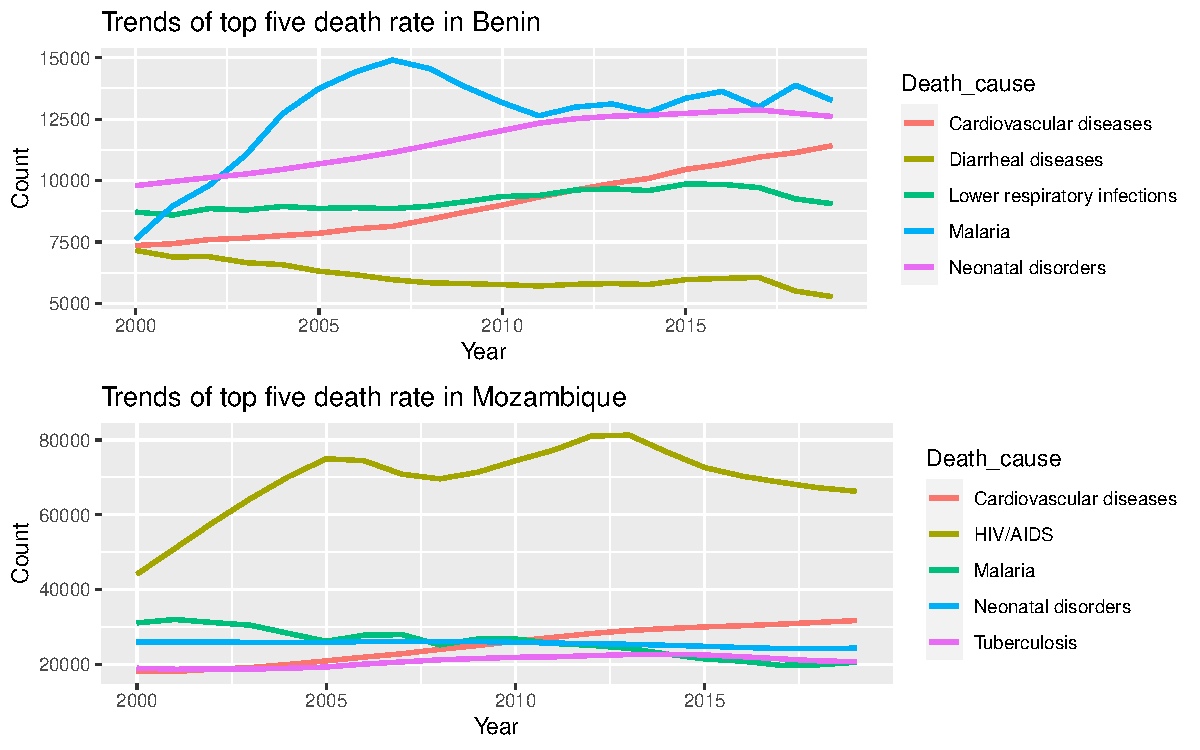
\includegraphics{Assignment4_files/figure-latex/topfiveplot-1.pdf}

According to figure graph\ref{fig:topfiveplot}, except Diarrheal disease, all the other four diseases were increasing from 2000 until now.Lower respiratory infections death reached the peak around 2015, and began to decrease in recent years.
For Mozambique, the death rate of Cardiovascular disease was increasing from 2000 until now. Death number for HIV and Tuberculosis reached the peak in around 2013 and began to drop.The death number of Malaria and Neonatal disorder was deceasing from 2000 until now.
In order to help these low-income countries get out of these difficulties, and save more life, high-income developed countries should help them by serving more medicines and vaccines. Also, more medical teams should support Africa and help patients in those low-income countries.
To make these tables and figure, I can also cite R packages as follows \textcite{tidyverse}, \textcite{ggplot2}, \textcite{readr}, \textcite{gridExtra}.

\hypertarget{conclusion}{%
\subsection{Conclusion}\label{conclusion}}

In conclusion, we can see that in high-income or developed countries like Australia, Switzerland, and Germany, the main death causes are cardiovascular diseases and they are caused by bad lifestyles and a long life time. People need to pay more attention to their mental health,and have a healthy diet. For those middle-income countries like China, India, and Mexico, the main death reason are cardiovascular and cancer, and the death reason is very related to the GDP of these countries. For those low-income countries, like Benin and Mozambique, people are suffering in many kinds of infectious diseases. We hope more high-income and developed countries can help those poor counties by severing more medical help, medicines and vaccines. All the countries in the world should collaborate with each other and make more people have happiness and healthy life.

\printbibliography

\end{document}
